\documentclass[notes,11pt, aspectratio=169]{beamer}

\usepackage{pgfpages}
% These slides also contain speaker notes. You can print just the slides,
% just the notes, or both, depending on the setting below. Comment out the want
% you want.
\setbeameroption{hide notes} % Only slide
%\setbeameroption{show only notes} % Only notes
%\setbeameroption{show notes on second screen=right} % Both

\usepackage{helvet}
\usepackage[default]{lato}
\usepackage{array}

\usepackage[backend=biber,style=authoryear,
sorting=ynt,citestyle=authoryear]{biblatex}
\addbibresource{Paper/papercitations.bib}

\usepackage{tikz}
\usepackage{verbatim}
\setbeamertemplate{note page}{\pagecolor{yellow!5}\insertnote}
\usetikzlibrary{positioning}
\usetikzlibrary{snakes}
\usetikzlibrary{calc}
\usetikzlibrary{arrows}
\usetikzlibrary{decorations.markings}
\usetikzlibrary{shapes.misc}
\usetikzlibrary{matrix,shapes,arrows,fit,tikzmark}
\usepackage{amsmath}
\usepackage{mathpazo}
\usepackage{hyperref}
\usepackage{lipsum}
\usepackage{multimedia}
\usepackage{graphicx}
\usepackage{multirow}
\usepackage{graphicx}
\usepackage{dcolumn}
\usepackage{bbm}
\newcolumntype{d}[0]{D{.}{.}{5}}
\usepackage{subfigure}
\usepackage{import}

\usepackage{changepage}
\usepackage{appendixnumberbeamer}
\newcommand{\beginbackup}{
   \newcounter{framenumbervorappendix}
   \setcounter{framenumbervorappendix}{\value{framenumber}}
   \setbeamertemplate{footline}
   {
     \leavevmode%
     \hline
     box{%
       \begin{beamercolorbox}[wd=\paperwidth,ht=2.25ex,dp=1ex,right]{footlinecolor}%
%         \insertframenumber  \hspace*{2ex} 
       \end{beamercolorbox}}%
     \vskip0pt%
   }
 }
\newcommand{\backupend}{
   \addtocounter{framenumbervorappendix}{-\value{framenumber}}
   \addtocounter{framenumber}{\value{framenumbervorappendix}} 
}

\setbeamertemplate{blocks}[rounded]
\setbeamercolor{block title}{bg=eggplant!70, fg=white}
\setbeamercolor{block body}{bg=eggplant!20}

\usepackage{graphicx}
\usepackage[space]{grffile}
\usepackage{booktabs}

% These are my colors -- there are many like them, but these ones are mine.
\definecolor{sage}{RGB}{102,153,102}
\definecolor{cambridgeblue}{RGB}{104, 166, 145}
\definecolor{yellow}{RGB}{255,173,1}
\definecolor{purple}{RGB}{153,102,153}
\definecolor{ashgray}{RGB}{191, 211, 193}
\definecolor{eggplant}{RGB}{105, 79, 93}
\definecolor{silver}{RGB}{192, 197, 193}
\definecolor{darkcyan}{RGB}{78, 135, 140}
\definecolor{lightcyan}{RGB}{201, 228, 231}
\definecolor{columbiablue}{RGB}{187, 213, 237}
\definecolor{lightblue}{RGB}{184, 219, 217}
\definecolor{earthyellow}{RGB}{234, 180, 100}

\setbeamercolor{mycolor}{fg=white,bg=sage}

% colors for diagrams
\definecolor{diagramtan}{RGB}{225,190,106}
\definecolor{diagramteal}{RGB}{64, 176, 166}
\definecolor{diagrampurple}{RGB}{170, 131, 239}
\definecolor{diagramred}{RGB}{146, 79, 79}


\hypersetup{
  colorlinks=false,
  linkbordercolor = {white},
  linkcolor = {sage}
}

\newcommand{\btVFill}{\vskip0pt plus 1filll}


%% I use a beige off white for my background
\definecolor{MyBackground}{RGB}{255,253,218}

%% Uncomment this if you want to change the background color to something else
%\setbeamercolor{background canvas}{bg=MyBackground}

%% Change the bg color to adjust your transition slide background color!
\newenvironment{transitionframe}{
  \setbeamercolor{background canvas}{bg=lightcyan}
  \begin{frame}[plain,noframenumbering]}{
    \end{frame}
}

\setbeamercolor{frametitle}{fg=black, bg=lightcyan}
\setbeamercolor{title}{fg=black}
\setbeamertemplate{footline}{%
  \raisebox{5pt}{\makebox[\paperwidth]{\hfill\makebox[15pt]{\scriptsize\insertframenumber}}}}
\setbeamertemplate{navigation symbols}{} 
\setbeamertemplate{itemize items}{$\bullet$}
\setbeamercolor{itemize item}{fg=lightcyan}
\setbeamercolor{itemize subitem}{fg=lightcyan}
\setbeamercolor{enumerate item}{fg=black}
\setbeamercolor{enumerate subitem}{fg=black}
\setbeamercolor{button}{bg=eggplant!20,fg=black}

\setbeamertemplate{frametitle}
{
    \nointerlineskip
    \begin{beamercolorbox}[sep=0.3cm,ht=2em,wd=\paperwidth]{frametitle}
        \vbox{}\vskip-2ex%
        \strut\insertframetitle\strut
        \vskip-0.8ex%
    \end{beamercolorbox}
}



% If you like road maps, rather than having clutter at the top, have a roadmap show up at the end of each section 
% (and after your introduction)
% Uncomment this is if you want the roadmap!
% \AtBeginSection[]
% {
%    \begin{frame}
%        \frametitle{Roadmap of Talk}
%        \tableofcontents[currentsection]
%    \end{frame}
% }

\setbeamercolor{section in toc}{fg=sage}
\setbeamercolor{subsection in toc}{fg=sage}
\setbeamersize{text margin left=1em,text margin right=1em} 

\newenvironment{wideitemize}{\itemize\addtolength{\itemsep}{10pt}}{\enditemize}

\usepackage{environ}
\NewEnviron{videoframe}[1]{
  \begin{frame}
    \vspace{-8pt}
    \begin{columns}[onlytextwidth, T] % align columns
      \begin{column}{.58\textwidth}
        \begin{minipage}[t][\textheight][t]
          {\dimexpr\textwidth}
          \vspace{8pt}
          \hspace{4pt} {\Large \sc \textcolor{blue}{#1}}
          \vspace{8pt}
          
          \BODY
        \end{minipage}
      \end{column}%
      \hfill%
      \begin{column}{.42\textwidth}
        \colorbox{green!20}{\begin{minipage}[t][1.2\textheight][t]
            {\dimexpr\textwidth}
            Face goes here
          \end{minipage}}
      \end{column}%
    \end{columns}
  \end{frame}
}

\title[]{\textcolor{sage}{Does Hospital Leadership Matter? \newline
Evidence from Pay-for-Performance}}

\author[]{Hanna Glenn}
\date{}


\begin{document}

%%% TIKZ STUFF
\tikzset{   
        every picture/.style={remember picture,baseline},
        every node/.style={anchor=base,align=center,outer sep=1.5pt},
        every path/.style={thick},
        }
\newcommand\marktopleft[1]{%
    \tikz[overlay,remember picture] 
        \node (marker-#1-a) at (-.3em,.3em) {};%
}
\newcommand\markbottomright[2]{%
    \tikz[overlay,remember picture] 
        \node (marker-#1-b) at (0em,0em) {};%
}
\tikzstyle{every picture}+=[remember picture] 
\tikzstyle{mybox} =[draw=black, very thick, rectangle, inner sep=10pt, inner ysep=20pt]
\tikzstyle{fancytitle} =[draw=black,fill=red, text=white]
%%%% END TIKZ STUFF

% Title Slide
\begin{frame}[plain]
% Background image
\begin{tikzpicture}[remember picture,overlay]
    \node
[
    above=0.5cm,
    align=center,
    fill=lightcyan,
    rounded corners,
    inner xsep=15pt,
    inner ysep=10pt, 
    minimum width=0.9\textwidth,
    text width=0.6\textwidth
] (title) at (current page.center)
{
    \LARGE Does Hospital Leadership Matter?  \\[5pt]
    \normalsize Evidence from Pay-for-Performance
};
% Author 
\node[below=1cm] (author) at (title.south){Hanna Glenn, Emory University};
% Date
\node[below=0.25cm] (date) at (author.south){\today};
\end{tikzpicture}
    
\end{frame}

\section{Intro}

\begin{frame}{Firm Leadership}
\centering
    \begin{tikzpicture}
        % First image (top-left)
        \node[anchor=north west] (img1) at (0, 3) {
\includegraphics[width=0.55\textwidth]{Graphics/theroleleadershiphasincompanyculture.png}};
        \draw[line width=.45mm, lightcyan] (img1.north west) rectangle (img1.south east);
        
        % Second image (slightly down and right of the first image)
        \node[anchor=north west] (img2) at (0.28, 0.58) {
\includegraphics[width=0.5\textwidth]{Graphics/linkingbusinessstrategyandleadershipforbetteroutcomes.png}};
        \draw[line width=.45mm, lightcyan] (img2.north west) rectangle (img2.south east);
    
        
        % Fourth image (bottom-right)
        \node[anchor=north west] (img4) at (0, -2) {
\includegraphics[width=0.55\textwidth]{Graphics/theroleofleadershipinorganizationalsuccess.png}};
        \draw[line width=.45mm, lightcyan] (img4.north west) rectangle (img4.south east);


    \end{tikzpicture}
\end{frame}

\begin{frame}{Leadership Characteristics}

\vspace{1mm}

\textbf{Gender}
\begin{itemize}
    \item \small More female board members $\implies$ lower firm value \scriptsize(\cite{ahern2012changing}) \small
    \item \small More female board members $\implies$ less employment reduction \scriptsize (\cite{matsa2013female}) \small
    \item female executives affect the female wage distribution \scriptsize (\cite{flabbi2019female}) \small
\end{itemize}

\vspace{2mm}

\textbf{Background}
\begin{itemize}
    \item \small Firms pay more for general background CEOs \scriptsize (\cite{custodio2013generalists}) \small
    \item \small CEOs w/ prior experience do better in M\&A \scriptsize(\cite{custodio2013ceos}) \small
    \item \small Military experience CEOs are less aggressive in R\&D and investing \scriptsize (\cite{benmelech2015military})
\end{itemize}

\vspace{2mm}

\textbf{Age}
\begin{itemize}
    \item \small Young male CEOs more aggressive in M\&A \scriptsize (\cite{levi2010deal})
\end{itemize}

\btVFill\pause

\begin{block}{\normalsize Gaps in Literature}
    \small 
    \begin{enumerate}
        \item Limited to large, publicly traded firms: reason to believe this does not extend to nonprofit setting
        \item Direct responses to policy changes are not well-understood
    \end{enumerate}
\end{block}
\end{frame}


\begin{frame}{Hospitals \& Health Care Policy Goals}

\begin{block}{This Paper}
    Examine the role of leadership in nonprofit hospitals responding to policy incentives 
\end{block}

\vspace{5mm}

\textbf{Hospital care makes up a third of health care spending} \scriptsize (\cite{cms2024nhe}) \normalsize
\begin{itemize}
    \item A majority of hospitals are nonprofit and their objectives are not as clear as classic for-profit firms
\end{itemize}

\vspace{5mm}

\textbf{Policies often aim to improve the value of health care delivery}

\vspace{3mm}

    \begin{wideitemize}
        \item It is unclear how hospital leaders view value
        \item Or whether they might play a role in achieving this goal
    \end{wideitemize}
\end{frame}

\begin{frame}{Research Question}
    \centering
    \large
    Does having executives with clinical training affect response to pay-for-performance incentives of nonprofit hospitals?
\end{frame}

\begin{frame}{Why Clinical Training?}

\textbf{Physician executives could be good or bad}

\vspace{2mm}

\begin{wideitemize}
    \item Physicians can bring a unique combination of clinical and administration expertise that can potentially lead to better quality \scriptsize (\cite{Stajduhar_2023}, \cite{Ahmed_2022}) \normalsize

    \vspace{2mm}
    
    \item Not always trained in business management, which can lead to poor practices and lower quality \scriptsize (\cite{HarvardBusinessReview2018})
\end{wideitemize}

\vspace{10mm}

\textbf{Clinical training is potentially correlated with how the leader values quality}
\end{frame}

\begin{frame}{Preview of Findings}

\textbf{Non-clinical executive teams respond more drastically to financial incentives on quality compared to clinical executive teams}

\vspace{2mm}

\begin{wideitemize}
    \item Non-clinical reduce readmissions by blank more than clinical
    \item Non-clinical executive teams behave like profit-driven hospitals
\end{wideitemize}
\end{frame}

\begin{frame}{Contribution}
    \textbf{Hospital Executives/Board of Directors}
    \begin{itemize}
        \item Physician board members $\implies$ lower public donations in nonprofit hospitals \scriptsize (\cite{brickley2010board}) \normalsize
        \item No correlation between CEOs and hospital production in England \scriptsize (\cite{janke2019impact})\normalsize
        \item Public hospitals in Chile improved when older physicians were removed as CEO \scriptsize (\cite{otero2022managers}) \normalsize
    \end{itemize}

    \vspace{5mm}

    \textbf{Hospital Response to Pay-for-Performance}
    \begin{itemize}
        \item Hospitals decreased readmissions by 40\% on average, partially due to selective patient practices \scriptsize (\cite{gupta2021impacts}) \normalsize
        \item Market concentration and systems affect response \scriptsize (\cite{kunz2024assessing}) \normalsize
        \item Reward program had little impact on quality \scriptsize (\cite{us2015hospital}; \cite{norton2018moneyball}; \cite{friedson2019so})
    \end{itemize}
\end{frame}

\begin{frame}{Rest of Talk}
    Theoretical Motivation

    \vspace{4mm}

    Setting and Data Collection

    \vspace{4mm}

    About Executive Teams

    \vspace{4mm}

    Effect of Clinical Leadership

    \vspace{4mm}

    Comparison to For-Profits

    \vspace{4mm}

    Signaling vs. Managing
\end{frame}



\section{Theoretical Framework}

\begin{transitionframe}
\centering \LARGE
    \textcolor{black}{Theoretical Framework}
\end{transitionframe}

\begin{frame}{Hospital Objectives}\label{hosp_obj}
\large
    \begin{equation*}
        \max_{\theta}\hspace{2mm}\alpha\pi(\theta) + (1-\alpha) u(\theta)
    \end{equation*}

    \vspace{5mm} \normalsize

    \begin{wideitemize}
        \item Profit $\pi$ and patient welfare $u$; depend on quality $\theta$
        \item Profit-driven hospitals have high $\alpha$
        \item Abstract away from quality impacting demand for care, price \hyperlink{complex_model}{\beamergotobutton{more complex model}} 
    \end{wideitemize}
\end{frame}

\begin{frame}{Choice of Quality}
Take FOC, rearrange and take derivative wrt $\alpha$:

\vspace{5mm}

\begin{equation*}
    \frac{du'(\theta)}{d\alpha} = \frac{-1}{(1-\alpha)^2}\pi'(\theta)
\end{equation*}

\vspace{5mm}

$\pi'(\theta)$:

\vspace{3mm}

\begin{wideitemize}
    \item In fee-for-service setting: negative $\implies \frac{du'(\theta)}{d\alpha} > 0$
    \item In pay-for-performance setting: positive $\implies \frac{du'(\theta)}{d\alpha} < 0$
\end{wideitemize}
    
\end{frame}

\begin{frame}{FFS $\implies$ P4P}
    \large
    \begin{align*}
        \frac{d\Delta\theta}{d\alpha}&=\frac{d\theta_{p4p}}{d\alpha}-\frac{d\theta_{ffs}}{d\alpha}\\ 
        &\\
        &=\frac{\frac{du'(\theta)}{d\alpha}}{\frac{du'(\theta)}{d\theta_{p4p}}} - \frac{\frac{du'(\theta)}{d\alpha}}{\frac{du'(\theta)}{d\theta_{ffs}}}\\
        &\\
        &> 0
    \end{align*}

    \btVFill \normalsize

    \begin{block}{Takeaway}
        Hospitals with higher weight on profit will respond more to the financial incentives on quality
    \end{block}
\end{frame}

\begin{frame}{Testable Predictions}
    \begin{enumerate}
        \item If non-clinical executives are more profit-driven than clinical executive hospitals, they will reduce quality by more

        \vspace{5mm}
        \item If non-clinical executives are more profit-driven, they will act more like for-profit hospitals 

        \vspace{5mm}
        \item Executive teams could reflect an underlying $\alpha$ or they could effectively change $\alpha$
    \end{enumerate}
\end{frame}

\section{Setting and Data Collection}

\begin{transitionframe}
\centering \LARGE
    \textcolor{black}{Setting and Data Collection}
\end{transitionframe}

\begin{frame}{Nonprofit Hospital Executives}\label{nonprofithospexec}
\textbf{What do executives do?}
\begin{wideitemize}
    \item Board of directors selects executives
    \item Executives handle the day-to-day operations of the hospital \hyperlink{executivejob}{\beamergotobutton{executive job}} 
\end{wideitemize}

\vspace{7mm}

\textbf{Executive teams}
\begin{wideitemize}
    \item Lots of variation in what executive teams look like
    \item Typically CEO and CFO, sometimes CMO 
\end{wideitemize}

\vspace{7mm}

Usable data on executives is rare
\end{frame}

\begin{frame}{}
    \begin{tikzpicture}
        % First image in the top-left
        \node[anchor=north west] at (0, 4) {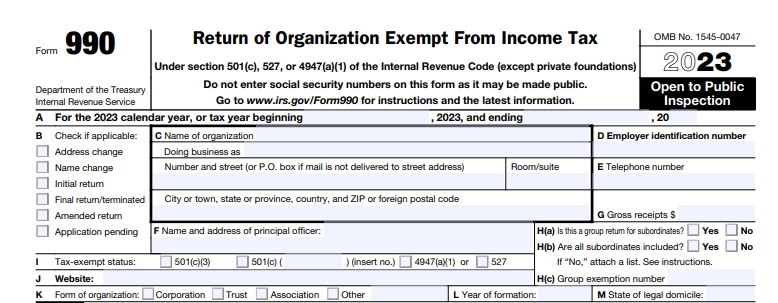
\includegraphics[width=0.7\textwidth]{Graphics/990_snip_frontpage.PNG}};
        % Second image in the middle
        \node[anchor=north west] (img2) at (2.5, 1.5) {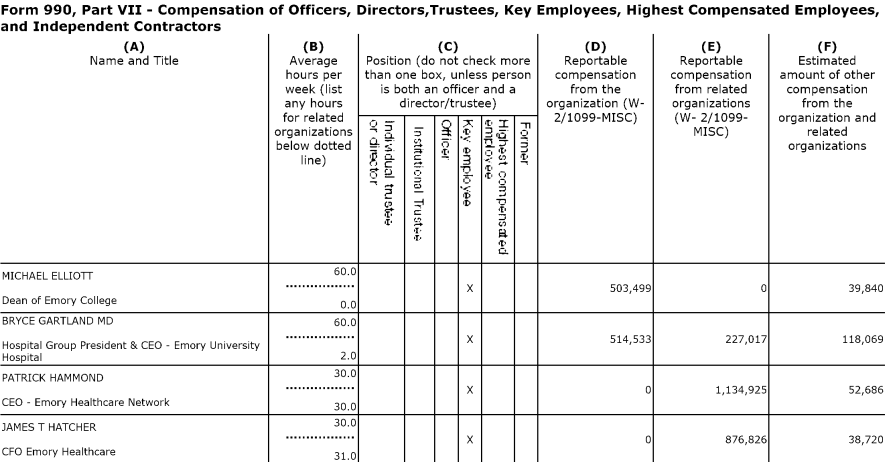
\includegraphics[width=0.75\textwidth]{Graphics/Screenshot 2024-10-03 160258.png}};
        \draw[line width=1mm, eggplant] (img2.north west) rectangle (img2.south east);
    \end{tikzpicture}
\end{frame}

\begin{frame}{Data Collection Process}
    \begin{enumerate}
        \item Get list of Employee Identification Numbers (EIN) that represent nonprofit hospitals

        \vspace{5mm}
        \item Download tax forms from 2009-2015 from Nonprofit Explorer API

        \vspace{5mm}
        \item Use Optimal Character Recognition to extract text from all of these documents

        \vspace{5mm}
        \item Write string cleaning algorithms to extract the correct name, title, position of each entry
    \end{enumerate}
\end{frame}

\begin{frame}{Merge to Other Hospital Data}
    I create links between EIN and ID number from the American Hospital Association Survey (AHA) based on hospital name and location

    \vspace{7mm}
    Merge to:

    \vspace{2mm}
    \begin{itemize}
        \item AHA data for hospital demographics
        \item Hospital Compare data for readmission and mortality rates
        \item Center for Medicare and Medicaid Services (CMS) Case Mix Index file for patient complexity
        \item Health Care Cost Report Information System (HCRIS) for information on pay-for-performance rewards or penalties
    \end{itemize}
\end{frame}

\begin{frame}{Merge to Physician Data}
    I use executives that self-identify as MD 

    \vspace{8mm}

    To verify, I match all executive names to database of all registered physicians and match NPI by hand
\end{frame}

\begin{frame}{About Pay-for-Performance Policies}
    Policies enacted in 2012 that either penalized for low quality or rewarded for high quality

    \vspace{3mm}

    \textbf{Hospital Readmissions Reduction Program}
    \begin{itemize}
        \item If hospitals have above average readmission rates they get 1-3\% lower reimbursement rates
        \item Pneumonia, Heart Attack (AMI), Heart Failure
    \end{itemize}

    \vspace{3mm}

    \textbf{Hospital Value-Based Purchasing Program}
    \begin{itemize}
        \item safety, efficiency, cost reductions, clinical outcomes, and community engagement, improvement combined into single score metric
        \item ``good" hospitals rewarded
    \end{itemize}

    \pause

    \begin{block}{\normalsize Takeaway}
        \normalsize All hospitals in the middle of the distribution had incentive to improve quality to try to avoid penalties, which were not perfectly predictable
    \end{block}
\end{frame}

\section{About Executive Teams}

\begin{transitionframe}
\centering \LARGE
    \textcolor{black}{Descriptive Statistics}
\end{transitionframe}

\begin{frame}{Executive Teams}
    \begin{table}[ht!]
        \centering
        \begin{tabular}[t]{lccc}
        \toprule
         & Ever & Always & Never\\
         & Clinical Exec & Clinical Exec &  Clinical Exec \\
        \midrule
        Number Executives & 4.85 & 5.25 & 3.11\\
        Frac Clinical Execs & 0.20 & 0.26 & 0\\
        Frac Int. Medicine Execs & 0.06 & 0.10 & 0.0\\
        Has a CMO & 0.53 & 0.45 & 0.15\\
        Has Clinical CEO & 0.25 & 0.11 & 0.0\\
        \addlinespace[0.6em]
        Num. Hospitals & 391 & 56 & 445\\
        \bottomrule
        \end{tabular}
    \end{table}
\end{frame}

\begin{frame}{Doctors on Executive Teams (N=813)}
    \begin{table}[ht!]
    \centering
    \begin{tabular}[t]{p{6cm} c}
    \toprule
     & Mean\\
    \midrule
    Age & 52.5\\
    Female & 0.11\\
    CEO & 0.16\\
    CMO & 0.31\\
    \addlinespace[0.3em]
    \multicolumn{2}{l}{\textbf{Specialty}}\\
    \hspace{1em}Internal Medicine & 0.32\\
    \hspace{1em}Family Medicine & 0.17\\
    \hspace{1em}Emergency Medicine & 0.11\\
    \hspace{1em}Surgery & 0.09\\
    \hspace{1em}Anesthesiologist & 0.04\\
    \hspace{1em}Other & 0.28\\
    \bottomrule
    \end{tabular}
    \end{table}
\end{frame}

\begin{frame}{Average Team Changes Over Time}
\centering 
    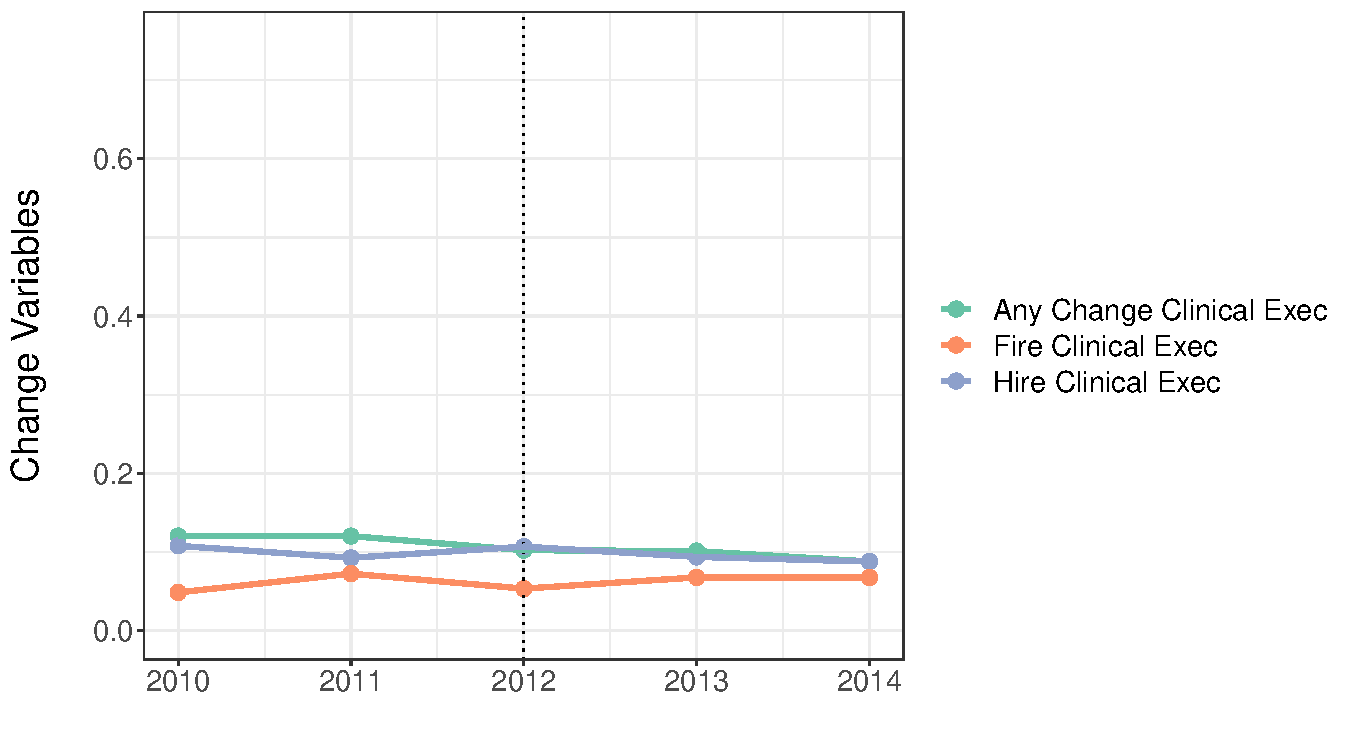
\includegraphics[width=.8\textwidth]{Objects/change_means.pdf}
\end{frame}

\begin{frame}{Changes are not correlated with policy exposure}
\centering \small
\begin{equation*}\label{eq:change2}
    \text{change}_{ht} = \sum_{j=2011}^{2014}\beta_j(\mathbf{1}\{t=j\}\times \text{Program Exposed})_{ht} + \alpha_h + \epsilon_{ht},
    \end{equation*}

    \btVFill

    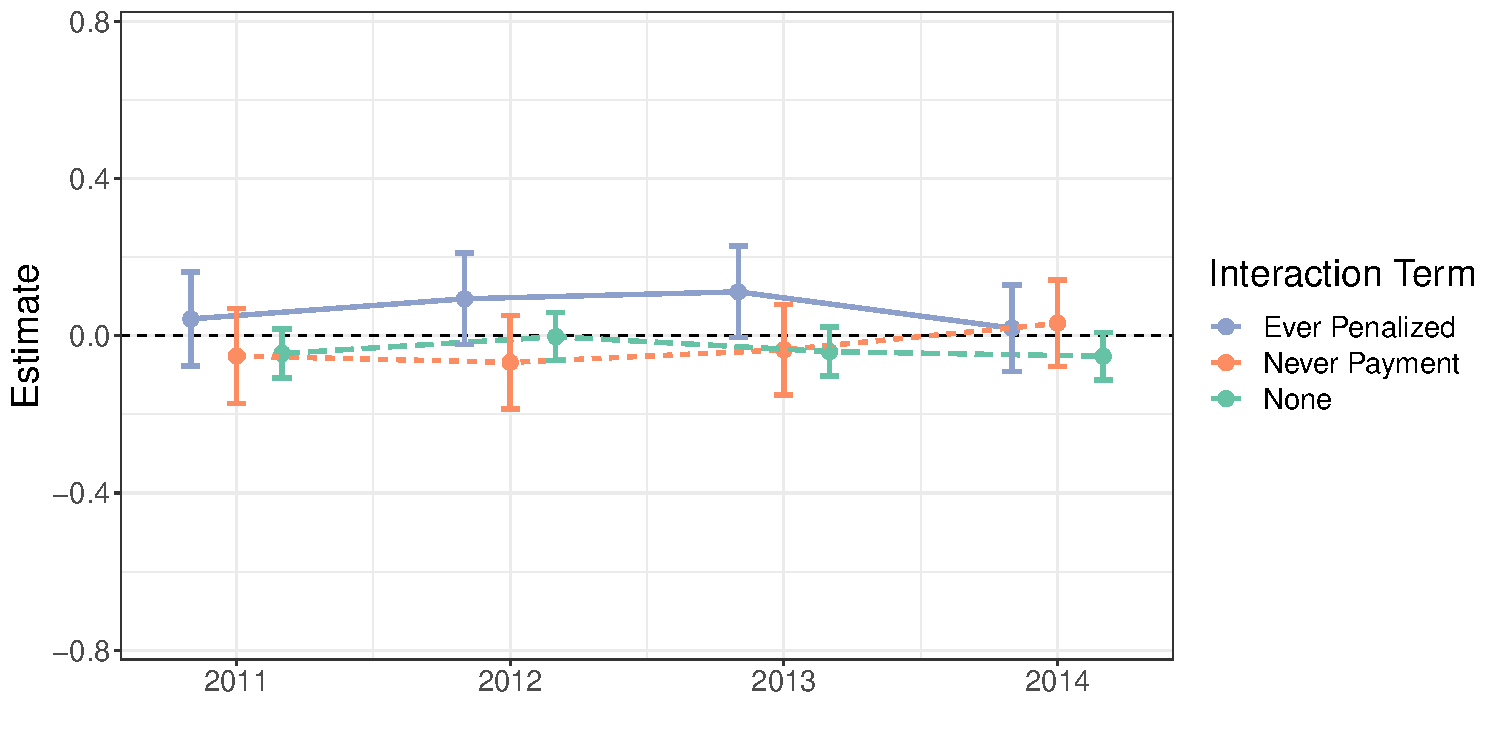
\includegraphics[width=.6\textwidth]{Objects/change_analysis_plot.pdf}
    
\end{frame}

\begin{frame}{Hospital Statistics}
\vspace{-2mm}
    \begin{table}[ht!]
    \centering
    \begin{tabular}[t]{lccc}
     & Ever & Always & Never\\
      & Clinical Exec & Clinical Exec & Clinical Exec\\
    \midrule
    \addlinespace[0.3em]
    \multicolumn{4}{l}{\textbf{Hospital Characteristics}}\\
    \hspace{1em}Academic Med. Center & 0.41 & 0.52 & 0.24\\
    \hspace{1em}Number Beds & 231 & 222 & 116\\
    \hspace{1em}Physician Owned & 0.01 & 0.02 & 0.02\\
    \hspace{1em}System Affiliated & 0.58 & 0.52 & 0.44\\
    \addlinespace[0.3em]
    \multicolumn{4}{l}{\textbf{Penalty/Payment Variables}}\\
    \hspace{1em}Ever Received HVBP Incentive & 0.79 & 0.75 & 0.62\\
    \hspace{1em}Penalized for One Condition & 0.18 & 0.20 & 0.13\\
    \hspace{1em}Penalized for AMI + HF/Pneum. & 0.09 & 0.09 & 0.06\\
    \hspace{1em}Penalized for HF + Pneumonia & 0.41 & 0.39 & 0.34\\
    \hspace{1em}Penalized for All Conditions & 0.30 & 0.27 & 0.22\\
    Num. Hospitals & 391 & 56 & 445\\
    \bottomrule
    \end{tabular}
    \end{table}
\end{frame}

\begin{frame}{}
    \includegraphics[width=\textwidth]{out}
\end{frame}


\section{Effect of Clinical Leadership on Response}

\begin{transitionframe}
\centering \LARGE
    \textcolor{black}{Effect of Clinical Leadership on Response}
\end{transitionframe}

\begin{frame}{Estimation}\label{est_equation}

    \vspace{5mm}\large
    \begin{equation*}
    y_{ht} = \beta \text{ (clinical training x post 2012)}_{ht} + \gamma_{h} + \delta_t + \epsilon_{ht}
    \end{equation*}
    \begin{itemize}
        \item Compare always to never clinical executives
        \item Leverage the timing of the programs
    \end{itemize}

    \vspace{8mm}

    Identifies the effect of having a clinically trained executive on readmission and mortality rates after pay-for-performance

    \vspace{2mm}
    
    \begin{itemize}
        \item Assume that hospitals would have had parallel trends absent clinical executives
    \end{itemize}

    \btVFill
    \normalsize
    \hyperlink{synthdid_equation}{\beamergotobutton{weighted}} \hyperlink{match_equation}{\beamergotobutton{matching}}
\end{frame}

\begin{frame}{Readmission Rates}\label{main:readrates}
\centering
    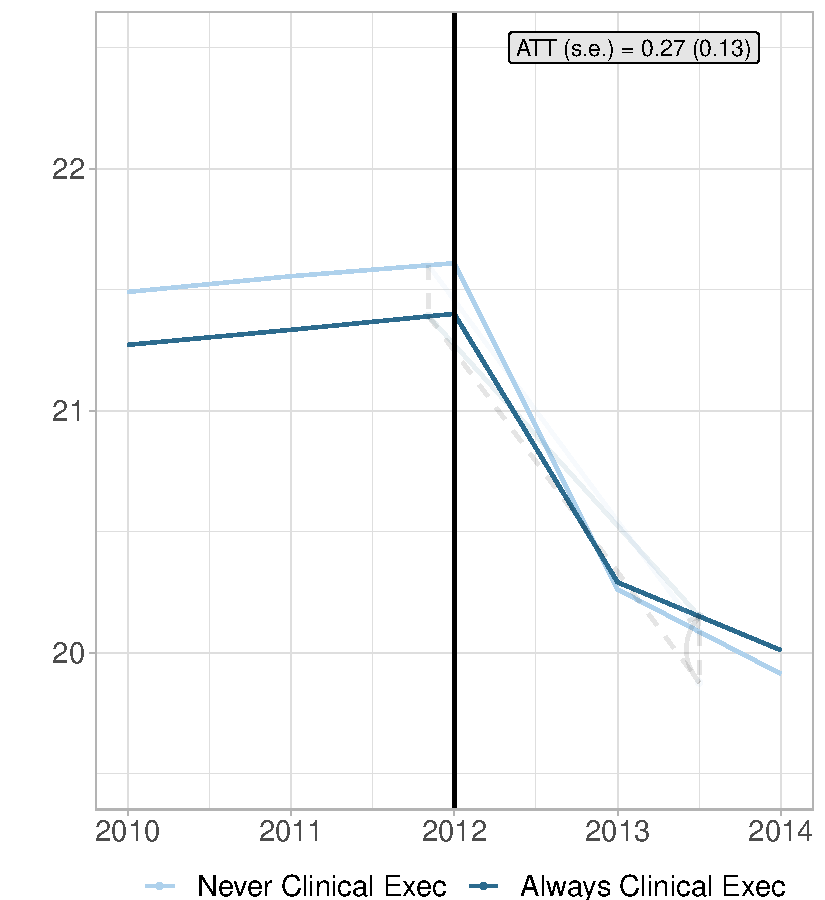
\includegraphics[width=.45\textwidth]{Objects/read_md_nomd_synth_graph.pdf}

    \btVFill
    
    \hyperlink{int_margin}{\beamergotobutton{intensive margin}}
\end{frame}

\begin{frame}{Mortality Rates}
    
\end{frame}

\section{Comparison to For-Profit Hospitals}

\begin{transitionframe}
\centering \LARGE
    \textcolor{black}{Comparison to For-Profit Hospitals}
\end{transitionframe}

\begin{frame}{Estimation}

    \vspace{5mm}\large
    \begin{equation*}
    y_{ht} = \beta \text{ (for-profit x post 2012)}_{ht} + \gamma_{h} + \delta_t + \epsilon_{ht}
    \end{equation*}
    \begin{itemize}
        \item Two comparison groups: clinical and non-clinical executive teams
    \end{itemize}

\end{frame}

\begin{frame}{Results}
    
\end{frame}

\section{Signaling vs. Managing}

\begin{transitionframe}
\centering \LARGE
    \textcolor{black}{Signaling vs. Managing}
\end{transitionframe}

\begin{frame}{Estimation}
    
\end{frame}

\begin{frame}{Results}
    
\end{frame}

\begin{frame}{Conclusion}
    
\end{frame}

\begin{frame}{Future Work}
    
\end{frame}

\begin{transitionframe}
\centering \Large
    \textcolor{black}{hkagele@emory.edu}
\end{transitionframe}




\section{Appendix}

\begin{transitionframe}
\centering \LARGE
    \textcolor{black}{Appendix Slides}
\end{transitionframe}

\appendix

\begin{frame}{More Complex Model}\label{complex_model}

\btVFill

\hyperlink{hosp_obj}{\beamerreturnbutton{hospital objectives}}
    
\end{frame}

\begin{frame}{Executive Job}\label{executivejob}

\btVFill

\hyperlink{nonprofithospexec}{\beamerreturnbutton{Nonprofit Hosp Execs}}
    
\end{frame}

\begin{frame}{Using synthetic DiD weights}\label{synthdid_equation}

\btVFill

\hyperlink{est_equation}{\beamerreturnbutton{main equation}}
    
\end{frame}

\begin{frame}{Matching}\label{match_equation}

\btVFill

\hyperlink{est_equation}{\beamerreturnbutton{main equation}}
    
\end{frame}

\begin{frame}{Intensive Margin}\label{int_margin}


    \btVFill

    \hyperlink{main:readrates}{\beamerreturnbutton{main results}}
\end{frame}


\end{document}

